
% !TEX TS-program = pdflatex
% !TEX encoding = UTF-8 Unicode

% This is a simple template for a LaTeX document using the "article" class.
% See "book", "report", "letter" for other types of document.

\documentclass[11pt]{article} % use larger type; default would be 10pt

\usepackage[utf8]{inputenc} % set input encoding (not needed with XeLaTeX)

%%% Examples of Article customizations
% These packages are optional, depending whether you want the features they provide.
% See the LaTeX Companion or other references for full information.

%%% PAGE DIMENSIONS
\usepackage{geometry} % to change the page dimensions
\geometry{a4paper} % or letterpaper (US) or a5paper or....
% \geometry{margin=2in} % for example, change the margins to 2 inches all round
% \geometry{landscape} % set up the page for landscape
%   read geometry.pdf for detailed page layout information

\usepackage{graphicx} % support the \includegraphics command and options

% \usepackage[parfill]{parskip} % Activate to begin paragraphs with an empty line rather than an indent

%%% PACKAGES
\usepackage{booktabs} % for much better looking tables
\usepackage{array} % for better arrays (eg matrices) in maths
\usepackage{paralist} % very flexible & customisable lists (eg. enumerate/itemize, etc.)
\usepackage{verbatim} % adds environment for commenting out blocks of text & for better verbatim
\usepackage{subfig} % make it possible to include more than one captioned figure/table in a single float
% These packages are all incorporated in the memoir class to one degree or another...

%%% HEADERS & FOOTERS
\usepackage{fancyhdr} % This should be set AFTER setting up the page geometry
\pagestyle{fancy} % options: empty , plain , fancy
\renewcommand{\headrulewidth}{0pt} % customise the layout...
\lhead{}\chead{}\rhead{}
\lfoot{}\cfoot{\thepage}\rfoot{}

%%% SECTION TITLE APPEARANCE
\usepackage{sectsty}
\allsectionsfont{\sffamily\mdseries\upshape} % (See the fntguide.pdf for font help)
% (This matches ConTeXt defaults)

%%% ToC (table of contents) APPEARANCE
\usepackage[nottoc,notlof,notlot]{tocbibind} % Put the bibliography in the ToC
\usepackage[titles,subfigure]{tocloft} % Alter the style of the Table of Contents
\renewcommand{\cftsecfont}{\rmfamily\mdseries\upshape}
\renewcommand{\cftsecpagefont}{\rmfamily\mdseries\upshape} % No bold!

\makeatletter
   \newcommand\figcaption{\def\@captype{figure}\caption}
   \newcommand\tabcaption{\def\@captype{table}\caption}
\makeatother
%%% END Article customizations

%%% The "real" document content comes below...

\title{CSE 509 Lecture 10}

\author{Prof. Rob Johnson, Scribe:Arun Rathakrishnan}
%\date{} % Activate to display a given date or no date (if empty),
         % otherwise the current date is printed 

\begin{document}
\maketitle
\section {Review}
Control flow automaton is based on static code analysis. Consider the below 
scenario.  

\begin{verbatim}
    func1(){
        ...
        func2();
        ...
    }
    func2(){
        ...
        ...
    }
    func3(){
        ...
        func2();	
        ...
    }
\end{verbatim}


func2 is a function that is often called by several functions in the application.
printf is one that is often called. In func1, func2 is called. The call sequence
is valid if the return of func2 is to the correct place in func1. However the
invalid sequence of returning to func3 (instead of func1) from func2 is accepted
by the model. The above model still does not prevent an attacker from forcing the
control to return to a function different from the caller and carry out an attack.
\section {Context Sensitive IDS}
Context Sensitive IDS  uses Context Free Grammars, represented by Push Down
Automata (PDA) to model the control flow in an application. By pushing on to a
stack an additional symbol ($1$ in case of func1 and $2$ in case of func2). We can
correctly define that a return to func1 is the only valid transistion by looking
at the top symbol. This plugs the weaknesses in Finite State Machine model.

\begin {center}
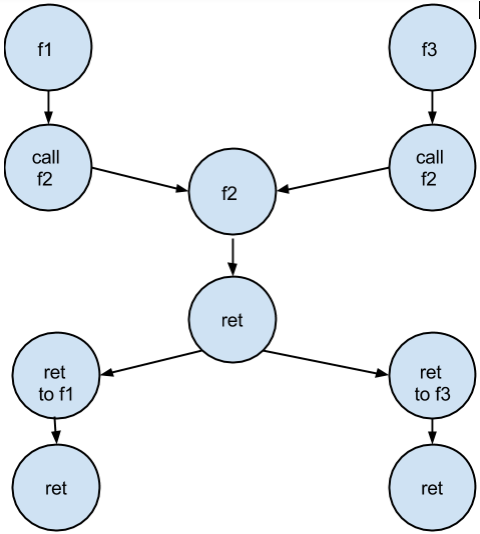
\includegraphics [width=220px,height=275px]{img/img2.png}\\
\caption{Control Flow Model}
\end {center}

\subsection {Verification}
The model of the application stores the PDA along with a stack and a state to
track the current state in a program. When a system call is made, it checks if
it is allowed from the current state (as in Finite State Machine Model) and
 pushes a symbol to the stack. On return, it pops the top character and makes
sure that the return is to the orginal caller. The weakness with this model is
ambiguity and explosion in number of states due to non-determinism.\\

After an if condition, there are two states where control can go. If there is
no sufficient information from the system call sequence to identify a particular
branch, we are left with no option than to bifurcate and keep track of both possible
stacks and states. At a later point, we will be able to spot the distinction
and discard the incorrect states. But before such a point is reached there can
be multiple branches thus exponentially increasing the amount of information to
be tracked.\\

Also since the model checking code runs in kernel, every time a function call is
made, a system call may be required to indicate a need to change the state or
stack which is a lot more costlier than actually making a function call in user 
space. This is a practical difficulty with the system.

\begin {center}
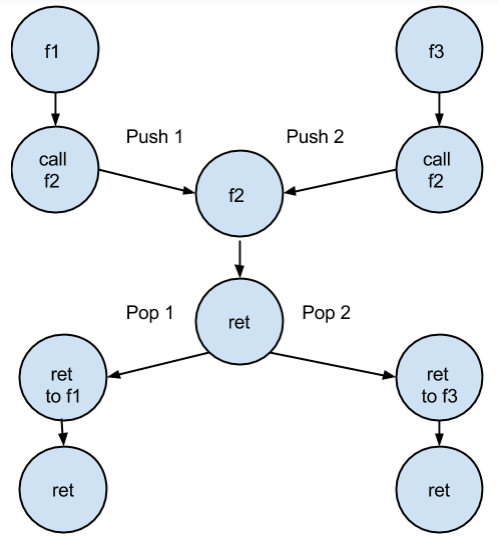
\includegraphics [width=220px,height=275px]{img/img1.png}\\
\caption {Pushing symbols to stack: PDA}
\end {center}

\subsection{How is this overcome?}
The binary is modified by adding a few instruction, so that model identifies a
branch that is taken after a conditional statement. The stack is represented as
a log, in the process address space. The controller keeps track of the last read
position in the call. The special instructions enable the process to push special
symbols that identify a branch. When a system call is made, the model checker pops
the marked position in the stack and from its current state, verifies if the
system can reach a state where the requested call can be allowed. This implementation
does away with the need to maintain a large number of states and stacks and
requires a system call (for the model checker to verify) only during when an
actual system call is made. Another unique feature is that the code is changed 
so as to assist the PDA to predict a branch. Log is in application memory and the
extra instructions write to this log.

\subsection {Exact model building}
Can we build a model that can perfectly predict the correct execution of a
program, so that it will accept only all possible sequences of system calls? 
If we can do that, the model effectively replaces the application and we can run
the model instead of the application.\\

Even if there were a model of computation that represented an application, we can
not decide by executing a model checker if its exactly equivalent to the current
application as the Equivalence problem of Turing Machines is undecidable.
It's unrealistic to expect a fool proof model that allows only the intended
system calls that an application can make.

\begin {center}
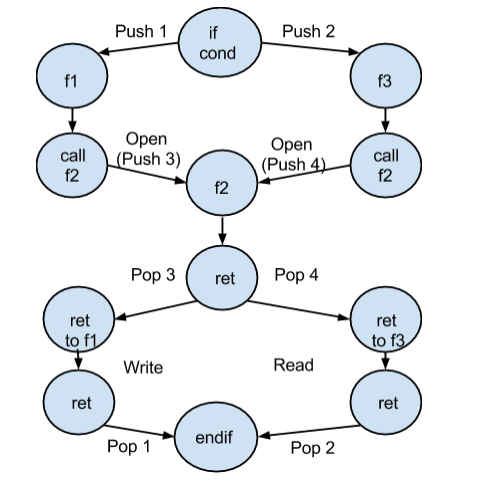
\includegraphics [width=220px,height=290px] {img/img3.png}\\
\caption {Non-determinsm}
\end {center}

\section {Memory Safe Compilation of C}
Ensures a program does not suffer from buffer overflow, even if the
source code or an input makes it possible. The main challenge is to ensure that
the pointer operations in a program are safe.

\begin {center}
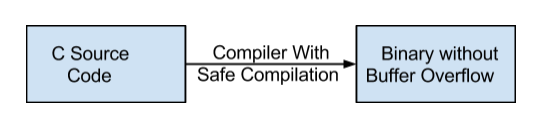
\includegraphics [width=270px,height=100px] {img/img4.png} \\
\caption {Memory Safe Compilation}
\end {center}

\subsection {Jones and Kelly Method}
Our goal: No pointer ever goes out of bounds.\\
Possible basic pointer operations:
\begin {itemize}\itemsep -2pt
\item Deference *p
\item Arithmetic q = p + n
\item Assignment q = p
\item Assignment, Typecast q = (char *)p
\item Malloc p = malloc(...);
\item Free free(p);
\item Assignment p = \&x;
\end {itemize}
Other complex operations can be written in terms of basic operations. Assume p[5]
can be rewritten as t = p+5; *t; in terms of the above operations.\\

If p is a safe pointer then q (on assignment) is also safe. Argument passing 
involves assigning actual parameters to local parameters, with similar operations.
So it can be treated as a special case, without making an extra check.

\begin{itemize} \itemsep -2pt
\item Track bounds for all objects.
\item Check all potentially dangerous pointer operations.
\end{itemize}

A data structure will be added to your program to track the bounds. This supports,
\begin{itemize} \itemsep -2pt
\item add(p, n): Allocation of a new object of size n at location p.
\item (low,hi) = lookup(p);
\end{itemize}
If there is no object in the queried range we can indicate that with a special 
values like $(0,0)$.
\\
subsection {Example Code}
\begin{verbatim}
    char * duplicate(char *p, int n){
        char * q = (char *) malloc(n);
        while(n--){
            *q++ = *p++;
        }
        return q-n;
    }
\end{verbatim}
\section {Review}
\begin{verbatim}
    char * duplicate(char *p, int n){
		*p = *q;
	}
\end{verbatim}



\begin{verbatim}
    char * duplicate(char *p, int n){
        (low, hi) = lookup(p);
        (low, hi) = lookup(q);
        assert(low <= p && p < hi);
        assert(low <= q && q < hi);
        *p = *q;
     }
\end{verbatim}
We do not perform the optimizations in the example for the sake of establishing
a simpler model.
Evaluation Criteria
Overheads:
1. Ten Times Slower in the original Jones and Kelly Model.
Baggy Bounds Techniqe
Look up table: Hash Table is not a suitable structure. Interval Tree is used. Splay trees were used.
2. Memory overhead. For each interval you have to store it in the interval tree node.
Not much of an overhead.
3. Effectiveness:
\section {Completeless Issues}
\subsection {Temporal Memory Safety}
Dangling Pointer
int * p = malloc();
free(p);
int * q = malloc();
*p = 5;

q may be allocated to the same address where p was allocated. Now this model
will not catch this as assertion will succeed.

struct foo{
    int a;
    int b;
};

\subsection {Intra-struct overflows}
struct foo * p = malloc();
q = p->a;
q = q + 1;
*q = 37;

Type confusion issues. J\&K method will not catch the type confusion errors, as
it does not consider anything about the internal structure.

\subsection {False Positives}
int A[10];
int *p = A;
for(i = 0; i < 10; ++i){
   *p = 0;
   p = p+1;
}

Modified Code:
int A[10];
insert(A,10);
lookup(p);
int *p = A;
for(i = 0; i < 10; ++i){
   (low, hi) = lookup(p);
   *p = 0;
   (low, hi) = lookup(p);
   assert(low <= p < high);
   (low, hi) = lookup(p+1);
   assert(low <= p+1 < high);
   p = p+1;
}

*-----------------------*
A                       A+10
i = 0                   p = A
i = 1                   p = A+1
i = 9                   p = A+9, p+1 = A+10

Assertion fails for p+1, when i = 9.
Another false positive as in Fig 2.
Needs to make sure that pointer never goes out of bounds. Or another object can
be overwritten. That's why there is a need for lookup after every assignment.

Separate compilation support.
Decisions made at one point should be independent of other files linked. J\&K is
good on separate compilation support. In fact, we need not know about another
line of code.
Linking transformed and untransformed code.
Some part of the library code may not be recompiled, so the application can
still have memory errors inside the untransformed code. The compiler can
insert some bounds checking before some functions like memcpy.
Pointer Laundering
Fig 4. Escapes assertions for bounds check in J\&K.
Recording allocations from library in uninformed. Can be fixed by changing the
malloc implementation and forcing the registration.

Criteria for evaluations
Runtime overhead
False Positives
EFfectiveness
Separate Compilation Support
Linking Transformed And Untransformed Code
No code changes

\section {Baggy Bounds Checking}
Has some similarity to J\&K. Bounds are kept for objects.
As a result pointers can not go out of bounds. 
Efficient lookups.
Efficient checks.
Main trick: Enable lookups using hashing.
Assumption: Smallest object that will be allocated is 16 bytes.
Assumption: All memory that will be allocated of $2^x$ bytes.
Assumption: Also aligned to $2^x$ that will be allocated is 16 bytes.
byte BNDS [$2^{32}/16$];
Only record the log of the size of memory allocated at any
location.
\end{document}
